\chapter{Modeling Cyber-Insurance }
\label{chp:modelingCyberInsurance} 


\section{Network Formation}


In many scenarios agents seeks to create networks in order to directly benefit from each other. The established links might represent companies out sourcing part of their manufacturing, or cooperative agreements in the development of new software products. In addition to increase the trade-off, each of the established links represents risk of being a victim of cascading failures. The intuitive example is the spread of epidemic diseases, also  (node failures of a power grid and) financial contagion such as the one back in 2008 was a result of cascading failures. Strategic network formation using cyber-insurance can be used to prevent such situation in addition to increase the overall payoff of participants in a clustered network.


When deciding whether to establish connection to a neighbour agent, the payoff has to be a balance between the expected earnings and the risk of the other party failing to complete the transaction. This is the reason why we seek to only download content from trusted peers and outlaw MC-gangs are consistently skeptical to enter into new agreements despite promising increased earnings, since the risk of undercover police are too high. 


In the paper \cite{contagion}, they come up with some interesting results regarding network formation games. 
They set up a game where the nodes benefit from direct links, but these links also expose them for risk. 
Each node gains a payoff of  $a$ per link it establishes, but it can establish a maximum of $\delta$ links.
A failure occur at a node with probability $q$, and propagates on a link with probability $p$. If a nodes fail, it will receive a negative payoff of $b$, no matter how many links it has established.

The results from their model shows a situation where clustered graphs achieve a higher payoff when connected to trusted agents, compared to when connecting with random nodes. Unlike in anonymous graphs, where nodes connect to each other at random, nodes in these graphs share some information with their neighbours, which is used when deciding whether to form a link or not. 
To further explain these results, they show that there exists a critical point, called phase transition, which occurs when nodes have a node degree of $1/p$. 
At this point a node gets a payoff of $a/p$, to further increase the payoff the node needs to go into a region with significantly higher failure probability. 
Because once each node establish more than $1/p$ links, the edges which propagates risk, will with high probability form a large cluster. Which results in a rise in probability of node failure, and reduces the overall wellfare.
From this the paper say that when the minimum welfare exceeds 
$(1+f(\delta)*a/p)$
we have reached super critical payoff. Otherwise it is called sub-critical payoff. 
Further they show that the only possible way of ending up with supercritical payoff, is by forming clustered networks consisting of cliques with slightly more than $1/p$ nodes. 
If the nodes form an anonymous market, random linking, they can only get sub-critical payoff. 
In other words, if the nodes can choose who they connect with, and by doing so, creating trusted clustered markets, they can achieve a higher payoff, by exceeding the critical node degree point. But in random graphs, this is not possible. 


Inspired by this model, we created a model which shields light on how cyber-insurance can be used in network formation to prevent cascading failures and increase an agents payoff.  



\section{Very Simple Model}

As a starting point the model is highly simplified in order to show the concept of how cyber-insurance can be used to create an insurable topology. Through out this chapter new features will be added to the model to make it more realistic and applicable. To begin, the model is formulated as follows.
A set of $n$ agents are randomly chosen to be insured or not. They all get their own fixed income, and by connecting to other agents they will receive a benefit resulting in higher payoff. Non-insured agents will have a risk of failure i.e. an expected cost of failure. Therefore if an insured agents chooses to connect to a non-insured agent they will also suffer from this expected cost of failure. In other words, the model follows a rule that insured agents are only willing to connect to other insured agents and non-insured agents can only connect with each other. In addition we apply the assumption that each node goes through the whole graph to decide whether to establish a connection or not. Since the decision is bidirectional, i.e. each agent must agree to establish the connection, the resulting graph will always be two fully connected cliques, one consisting of a insured agents and the other of non-insured agents. 


This dichotomy represents a trusted environment for the insured nodes, because they are able to trust each other since everyone is protected from risks such as financial catastrophe. These agents will benefit from each connection without having to worry about contagious risks from the connected agents. 
An agent in the non-insured clique will also receive the aggregated benefits from the connections, however each of the connection has a probability of failure. Hence this environment is not trusted, and a decision on whether to connect always involves some risks. 

\begin{figure}[h]
\centering
\begin{subfigure}{.5\textwidth}
  \centering
  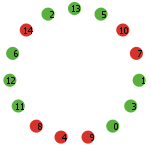
\includegraphics[width=0.4\linewidth]{../Figures/firstModelWithNoParameters1.png}
  \caption{\label{fig:firstmod1} 15 Agents randomly choosen to be either insured (green) or non-insured (red.}
\end{subfigure}
\quad
\begin{subfigure}{.46\textwidth}
  \centering
  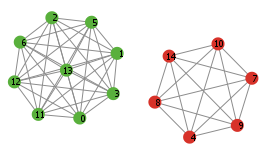
\includegraphics[width=0.8\linewidth]{../Figures/firstModelWithNoParameters2.png}
  \caption{\label{fig:firstmod2} Two clustered networks. One consisting of insured agents the other consists of non-insured.}
\end{subfigure}
\caption{\label{fig:fincont} shows how insured agents connects with each other to form a network to achieve super-critical payoffs.}
\end{figure}

In many situations agents, such as companies are in a situation where they have to establish connections. One example can be a non-insured company needing to outsource certain tasks to remain competitive, if all the potential companies for outsourcing are insured, the company will have a strong incentive to also buy insurance in order to be able to establish a connection. Hence this model, although very simple, shows an insurable topology where insured agents benefit from being insured. 

There are some limitations of the model, among others it fails to reflect the dynamics of a real world scenario, where each node will have different variables with different values. In addition, each node have a complete overview of the other nodes status. i.e. the problem with information asymmetry is not taken into account. 

\subsection{Model with parameters}
To make this simple model more realistic, we have to create a game with parameters, The characteristics of the game is as follows: an agent can be either insured or not insured, the insured ones have to pay an insurance cost $I_{0}$. Every agent starts with a fixed income, $\alpha$, to further increase their income they have to establish links to other agents. For each link they establish they receive a payoff of $\beta$. An insured node has to pay a cost of $I_{l}$ for every link he establish. The game is bidirectional, so both agents has to agree to the establishment of a link, and if both are insured, they both have to pay the cost $I_{l}$. 
Every agent who is not insured will have a risk of failure(infected, bankruptcy, or some other type of failure), this is captured with the expected risk cost $r$. Every node who connects to an node who is not insured will also suffer from this cost. See Table \ref{tbl:simplegamepara} for an overview of the parameters. 
\begin{table}[h]
\centering
\begin{tabular}{lc}
 \hline
  $\alpha$ - agents fixed income\\
  $\beta$ - income from establishing a direct link \\
  $I_{o}$ - cost of having insurance. \\
  $I_{l}$ - increased insurance cost per link the node establishes\\
  $r$ - expected risk cost\\
  \hline
\end{tabular}
\caption{Table showing the parameters to be used in the first model \label{tbl:simplegamepara}}
\end{table}
\subparagraph{Two agent game}
To begin analysing this game, lets consider a two-person game at first. In this game the strategy space of both players consist of four different strategies. They can choose insurance or not, and to establish link or not. I.e. the different strategies are: be insured and establish link noted as: $IL$, 
be insured and do not establish link: $I\overline{L}$. Not insured and establish link: $\overline{I}L$, and not insured and do not establish link: $\overline{IL}$.
Figure \ref{fig:FirstGameTheoryModel} shows the different outcomes of this game.

\begin{figure}[h]
\centering
\begin{tabular}{@{}c@{}}
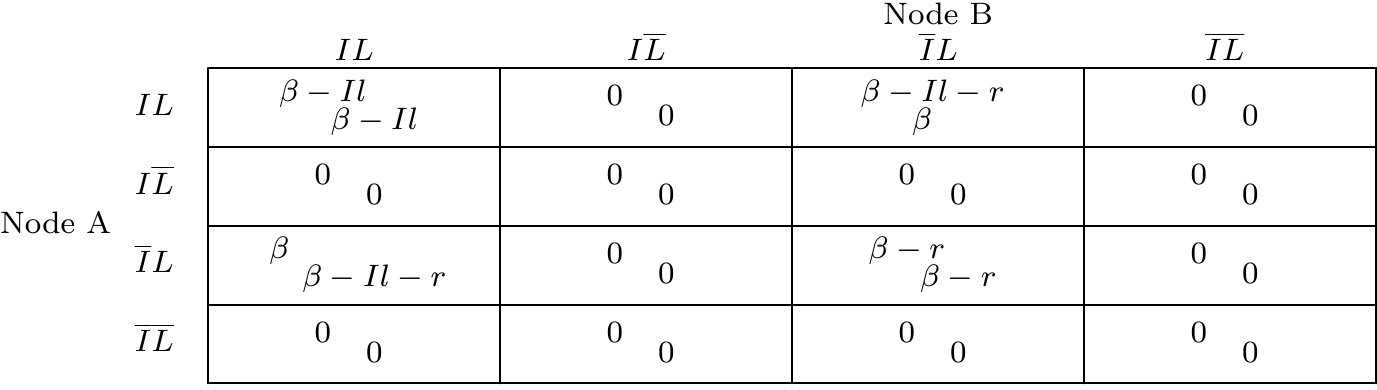
\includegraphics[width=1.0\textwidth]{../Figures/FirstGameWithParameters.png}
\end{tabular}
\caption{\label{fig:FirstGameTheoryModel} Normal form game, showing the different strategies and the payoffs  for the different outcomes. The payoff for agent A is written first, then the payoff for agent B is on the line beneath.
 An agent has a strategy space of size 4. }
\end{figure}

The simple game described earlier where the insured nodes form a trusted clique is what we want to achieve. 
When non-insured nodes connect to each other, they both end up with this payoff \ref{eq:notinsured payoff}. If they do not establish connection, they both receive the payoff \ref{eq:notinsured payoff2}.
\begin{equation}
U_{i}=\alpha - 2*r +\beta
\label{eq:notinsured payoff}
\end{equation}
\begin{equation}
U_{i}=\alpha - r
\label{eq:notinsured payoff2}
\end{equation}
From this equation we see that if $r>\beta$ then no connections will be made between non-insured agetents, because then they would strictly prefer the payoff from not connecting.
If a insured agent connects to an non-insured one, he will end up with this payoff \ref{eq:insured-noninsured}. If he dont connect he will receive this payoff \ref{eq:insured-noninsured2}.
\begin{equation}
U_{i}=\alpha - I_{0} - I_{l} - r + \beta
\label{eq:insured-noninsured}
\end{equation}
\begin{equation}
U_{i}=\alpha - I_{0}
\label{eq:insured-noninsured2}
\end{equation}
As we see if $I_{l}+r>\beta$ the insured one will prefer not to connect, if not he will establish connection, and since the non-insured agent is always better off when connected to an insured agent, he will accept the establishment. This is easy to see when comparing the two payoffs. Payoff of connecting to a insured one: $U_{i}=\alpha - r + \beta$ is allways higher than not connecting: $U_{i}=\alpha - r$ this holds as long as $\beta>0$.
To ensure that only insured nodes connect to each other, we want \ref{eq:insured-noninsured2} to be larger than \ref{eq:insured-noninsured}. I.e. This has to hold:
\begin{equation}
I_{l}+r>\beta
\label{eq:condition}
\end{equation}
When insured nodes connect to other insured nodes, they both end up with this payoff:
\begin{equation}
U_{i}=\alpha - I_{0} - I_{l} + \beta
\label{eq:insured-insured}
\end{equation}
To ensure that both agents will connect to each other this has to hold:
 \begin{equation}
I_{l}<\beta
\label{eq:condition2}
\end{equation}
For the game to end up as the one described earlier, where only insured nodes connect to other insured nodes, both \ref{eq:condition} and \ref{eq:condition2} has to hold, which gives us this limitation on the parameter $I_{l}$:
\begin{equation}
\beta-r<I_{l}<\beta
\label{eq:final condition}
\end{equation}
For the non-insured nodes to connect to each other, the only condition is that $\beta>r$. As long as these limitation is fulfilled, the game will end up with insured agents only establishing connections to other insured nodes, and non-insured nodes only connecting to non-insured nodes. It is easily seen that this holds for the two-agent game but also when there are multiple agents in the game.

In this model the network formation is done endogenously, and when following the limitation \ref{eq:final condition} we ensure that only insured nodes will connect, and we end up with an insurable network topology. 
In this model we have neglected the information problem, we assume that all nodes can differentiate insured versus non insured nodes. This could be difficult to realize in many real world network, but in financial transactions and in software development networks, it is reasonable to assume that the parties can acquire this type of information regarding their transactional partners. And thus they solve the information asymmetry problem by them self, by requiring proof of insurance prior to establishing a connection. This will result in insurable-clustered components  evolve endogenously in the network. Which is beneficial for both the insurer and the nodes.

\subparagraph{Example scenario}
By assigning values to the variables, we can show the outcome of the game in different scenarios. With the values from \ref{tbl:simplegamevalue}, the insurance cost of establishing a link satisfies the condition in equation \ref{eq:final condition}.
If we play this game between two agents we can see the result in the normal form table:\ref{fig:NFnumbers}. 
We see that the results are as we expected, insured nodes will only choose to connect with other insured nodes, they are also satisfied when not connected to each other, but this is not the social optimal outcome, and since they have complete network information, they will choose to connect to each other, because they will both achieve receive a higher payoff.
As we know, it does not matter if we consider only a two person game, because the change in payoffs when adding a link, is linear an independent of the agents degree, thus no insured agents will connect to non-insured ones.
\begin{table}[h]
\centering
\begin{tabular}{lc}
 \hline
  $\alpha=10,
  \beta=10,
  I_{o}=5,
  I_{l}=3,
  r=8$\\
  \hline
\end{tabular}
\caption{Table showing the parameters and their assigned values \label{tbl:simplegamevalue}}
\end{table}

\begin{figure}[h]
\centering
\begin{tabular}{@{}c@{}}
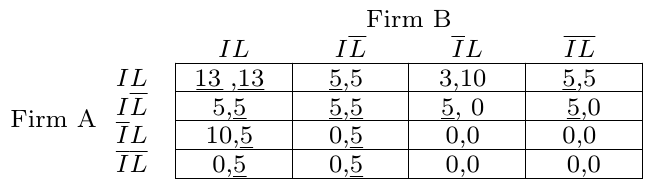
\includegraphics[width=1.0\textwidth]{../Figures/gameTheoryModel1WithNumbers.png}
\end{tabular}
\caption[Caption for LOF]{Normal form game between two agents with the parameters given in \ref{tbl:simplegamevalue}, the best response of a player to a given strategy is marked with an underscore.There are two pure nash equilibriums in this game,$IL,IL$ and $I\underline{L},I\underline{L}$. \label{fig:NFnumbers}}
\end{figure}
When setting the insurance cost: $I_{l}<\beta - r$ or $I_{l}>\beta$ we are violating the condition who ensured that only insured nodes connected to each other. The results are shown in Figure \ref{fig:NFnumbersViolating}. As we see there are still the same nash equilibrium, but whats interesting is the best response of an insured agent when the other agent is not insured, and both choose to establish link. This scenario has now changed, and we see that the insured agent would agree to the link establishment, this could result in an untrusted and thus an non-insurable topology. Therefore to ensure that only insured agents connect to each other, equation \ref{eq:final condition} has to be satisfied. 
In this particular situation with only two agents, the game will still end up in one of the nash equilibriums and only insured will connect to insured. But imagine a situation with more agents, then the insured node will also connect to the non-insured ones, and thus create a non-trusted network(non-insurable topology).
\begin{table}[h]
\centering
\begin{tabular}{lc}
 \hline
  $\alpha=10,
  \beta=10,
  I_{o}=5,
  I_{l}=1,
  r=8$\\
  \hline
\end{tabular}
\caption{Table showing the parameters and their assigned values, the insurance cost of establishing link is now violating the equation \ref{eq:final condition} \label{tbl:simplegamevalue2}}
\end{table}

\begin{figure}[h]
\centering
\begin{tabular}{@{}c@{}}
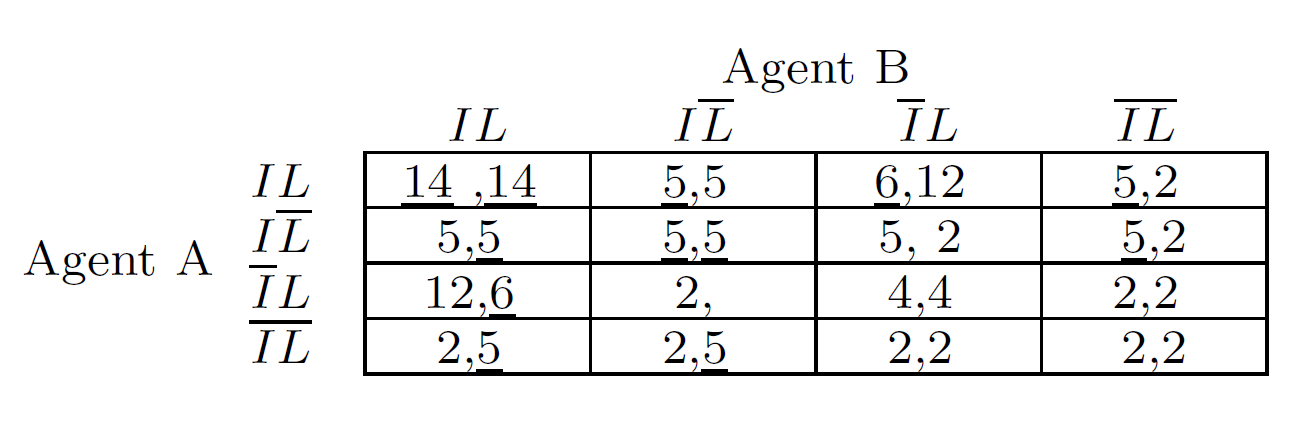
\includegraphics[width=1.0\textwidth]{../Figures/NotOptimalGameWithNumbers.png}
\end{tabular}
\caption[Caption for LOF]{Normal form game between two agents with the parameters given in table \ref{tbl:simplegamevalue2}, the best response of a player to a given strategy is marked with an underscore.There are two pure nash equilibriums in this game,$IL,IL$ and $I\underline{L},I\underline{L}$. \label{fig:NFnumbersViolating}}
\end{figure}
\subsection{Modelling the game with different parameters and multiple agents}

To see the outcomes of this game more clearly and to verify the multiple agent scenarios, we created a simulator that models the scenario. The rules are as described earlier, when a node is considering establishing a link it chooses to do so if the payoff it will receive is larger than the payoff it have when not establishing the link, and the decision is bilateral. 
In the simulator a node is insured with a probability, $p$. The network formation is performed by selecting two random nodes, not neighbouring each other, then both nodes checks if they would prefer to establish a connection or not. This selection is repeated until the network are fully connected or no more nodes are willing to establish new connections.
\subparagraph{Simulation of game with optimal parameters}
\begin{figure}[h]
\centering
\begin{subfigure}{.5\textwidth}
  \centering
  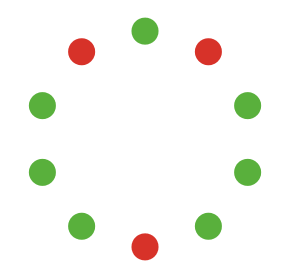
\includegraphics[width=0.4\linewidth]{../Figures/FirstSimulationStart.png}
  \caption{\label{fig:firstsimulationstart} Ten nodes randomly, with probability 0.5, chosen to be either insured (green) or non-insured (red.}
\end{subfigure}
\quad
\begin{subfigure}{.46\textwidth}
  \centering
  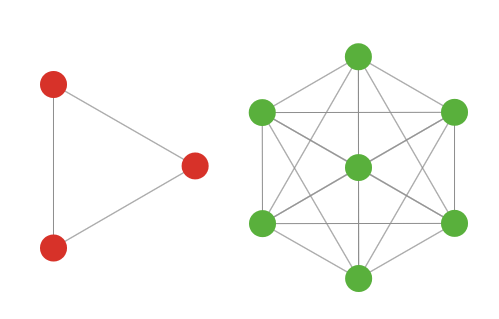
\includegraphics[width=0.8\linewidth]{../Figures/FirstSimulationResult.png}
  \caption{\label{fig:firstsimulationresult} Two clustered fully connected networks. One consisting of insured agents the other consists of non-insured. The link establishment is done by following the rules described above}
\end{subfigure}
\caption{\label{fig:firstsimulation} The figure shows how ten nodes start out with no links, and then add links as long as they can increase their payoff, the result are two seperate cliques, one consisting of non-insured and the other of insured nodes.}
\end{figure}
In figure \ref{fig:firstsimulation} we see the result of a simulation with the parameters from table \ref{tbl:simplegamevalue}, with these parameters the game should end in two cliques, one with insured nodes and another with non-insured. The result are shown in figure \ref{fig:firstsimulationresult}. Our calculations where confirmed, only insured nodes connect to each other.  
In this figure there are only included $n=10$ nodes, this is done to make the figure understandable and readable.
The same results where confirmed when performing the simulation with larger values of n, but the resulting picture was very complex and chaotic.
\subparagraph{Simulation of game with parameters violating equation \ref{eq:final condition}}
\begin{figure}[h]
\centering

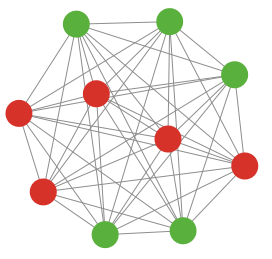
\includegraphics[width=0.4\textwidth]{../Figures/FirstSimulationViolatingResult.png}

\caption{\label{fig:SimulationViolating} Ten nodes insured with probability 0.5, and the parameters from table \ref{tbl:simplegamevalue2}. The link insurance cost, $I_{l}$, is violating the condition in equation \ref{eq:final condition}, and the resulting network is one clique of both insured and non-insured nodes.}
\end{figure}

\subsection{DETTE ET ANNET STED KANSKJE? BLIR LITT RART Å HOPPE INN I DET HER}
By adjusting the parameter one can assure that only insured agents connects to other insured agents, and the opposite,
that only uninsured agents connects to each other. Hence as we can see from the figure \ref{fig:fincont} clustered
networks of insured agents (red) are created, and  as the paper \cite{contagion} showed, these clustered trusted
networks, can achieve higher, super-critical, payoff by increasing their node degree past the critical point.

\begin{figure}[h]
\centering
\begin{subfigure}{.5\textwidth}
  \centering
  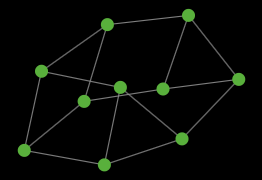
\includegraphics[width=0.8\linewidth]{../Figures/financialContagion1.png}
  \caption{\label{fig:fincont1} Initial graph with 10 agents.}
\end{subfigure}
\quad
\begin{subfigure}{.46\textwidth}
  \centering
  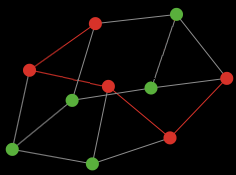
\includegraphics[width=0.8\linewidth]{../Figures/financialContagion2.png}
  \caption{\label{fig:fincont2} Insured agents (red) forms a network}
\end{subfigure}
\caption{\label{fig:fincont} shows how insured agents connects with each other to form a network to achieve super-critical payoffs.}
\end{figure}

, because the nodes can thus receive a super-critical payoff, and they are also insured against contagious risk.  

Figure \ref{fig:GTmodel1equations} presents the individual payoffs in a formation game between two agents in the described model. It is assumed that both agents has to have a desire to establish a connection in order to create a link between them. This is reasonable since a company would not prefer to enter into an agreement with negative expected payoff. As in this case would be the result when an insured agent is requested a connection with someone without insurance. 
 
 
\begin{figure}[h]
\centering
\begin{tabular}{@{}c@{}}
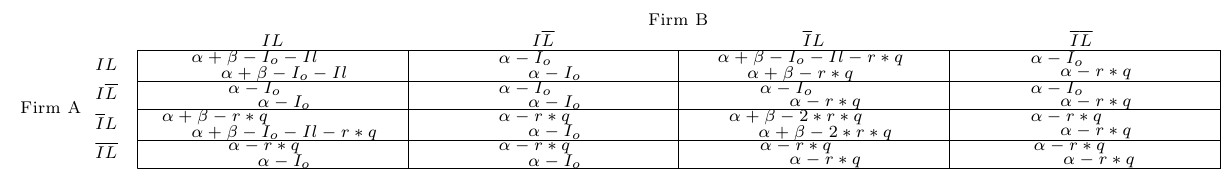
\includegraphics[width=1.0\textwidth]{../Figures/gameTheoryModel1WithEquations.png}
\end{tabular}
\caption[Caption for LOF]{\label{fig:GTmodel1equations} Normal form game between two agents individually choosing to purchase insurance and express desire to connect to the other  \footnotemark }
\end{figure}
\footnotetext{A link will only be created if both agents wishes to establish a connection.}

If we give value to the variables in figure \ref{fig:GTmodel1equations} one can observe the model's different equilibrium's. It is difficult to know exactly how the variables are set and this would vary considerably between different markets. In a real worlds scenario the variables would also be different for each agent. However in figure \ref{fig:GTmodel1} we decided to set a fixed value (which is assumed to be corresponding to the real values) for each variable in order to show a concept of how cyber-insurance can be used to create beneficial payoffs.
The following values where used: $\alpha$ = 10, $\beta$ = 10, $I_{o}$ = 5, $I_{l}$ = 2, $r$  = 20, $q$ = 0.5.


\begin{figure}[h]
\centering
\begin{tabular}{@{}c@{}}
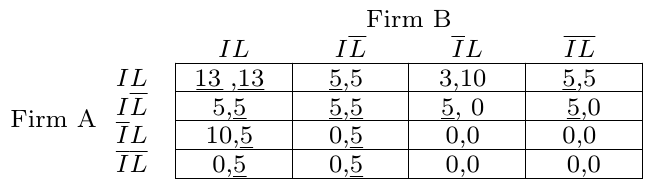
\includegraphics[width=0.6\textwidth]{../Figures/gameTheoryModel1WithNumbers.png}
\end{tabular}
\caption{\label{fig:GTmodel1} Shows equilibrium's in the resulting payoff matrix.}
\end{figure}

From the payoff matrix \ref{fig:GTmodel1} we observe two different Nash equilibrium's: One when both agents are insured and wants to connect to the other agent, and one when both are insured but does not want to establish a connection. These are the possible outcomes between the two agents, however as we can see it the social optimal solution would be for two insured agents to connect with each other, i.e they would both receive a significantly higher payoff. This demonstrates that a cluster of insured nodes would achieve higher payoffs.  
